% Largeur commune des logos : en fixant une valeur absolue (cm),
% les deux logos auront exactement la même largeur à l'affichage,
% quelle que soit la résolution ou le ratio de l'image source.
\newcommand{\logowidth}{3.2cm}

\begin{titlepage}
    \centering
    \vspace*{-1.2cm} % remonte l'ensemble du bloc de logos vers le haut de la page

    % ---- Ligne des logos (alignés en haut grâce à [t]) ----
    \noindent
    \begin{minipage}[t]{0.48\textwidth}
        \raggedright
        
\includegraphics[width=\logowidth]{logos/IPSA_LOGO_2024_QUADRI.png}\\[0.3cm]
        \textbf{\textsc{Institut Polytechnique des Sciences Avancées}} \\
        \small 81 Av. de Grande-Bretagne \\
        \small 31300 Toulouse, France 
    \end{minipage}
    \hfill
    \begin{minipage}[t]{0.48\textwidth}
        \raggedleft
        
\includegraphics[width=6.5cm]{logos/ONERA_logo.png}\\[0.3cm]
        \textbf{\textsc{Office National d'Études et de Recherches Aérospatiales}}\\
        \small 2 Av. Marc Pélegrin,  \\
        \small 31400 Toulouse, France
    \end{minipage}

    \vspace{1.2cm}

    % ---- Titre du rapport ----
    {\Large \textbf{Rapport PMI}} \\
    \vspace{0.5cm}
    {\Huge \textbf{Reconstitution de données d'environnement spatial}}
    \vspace{5mm}

    % ---- Image centrale ----
    \begin{figure}[h]
        \centering
        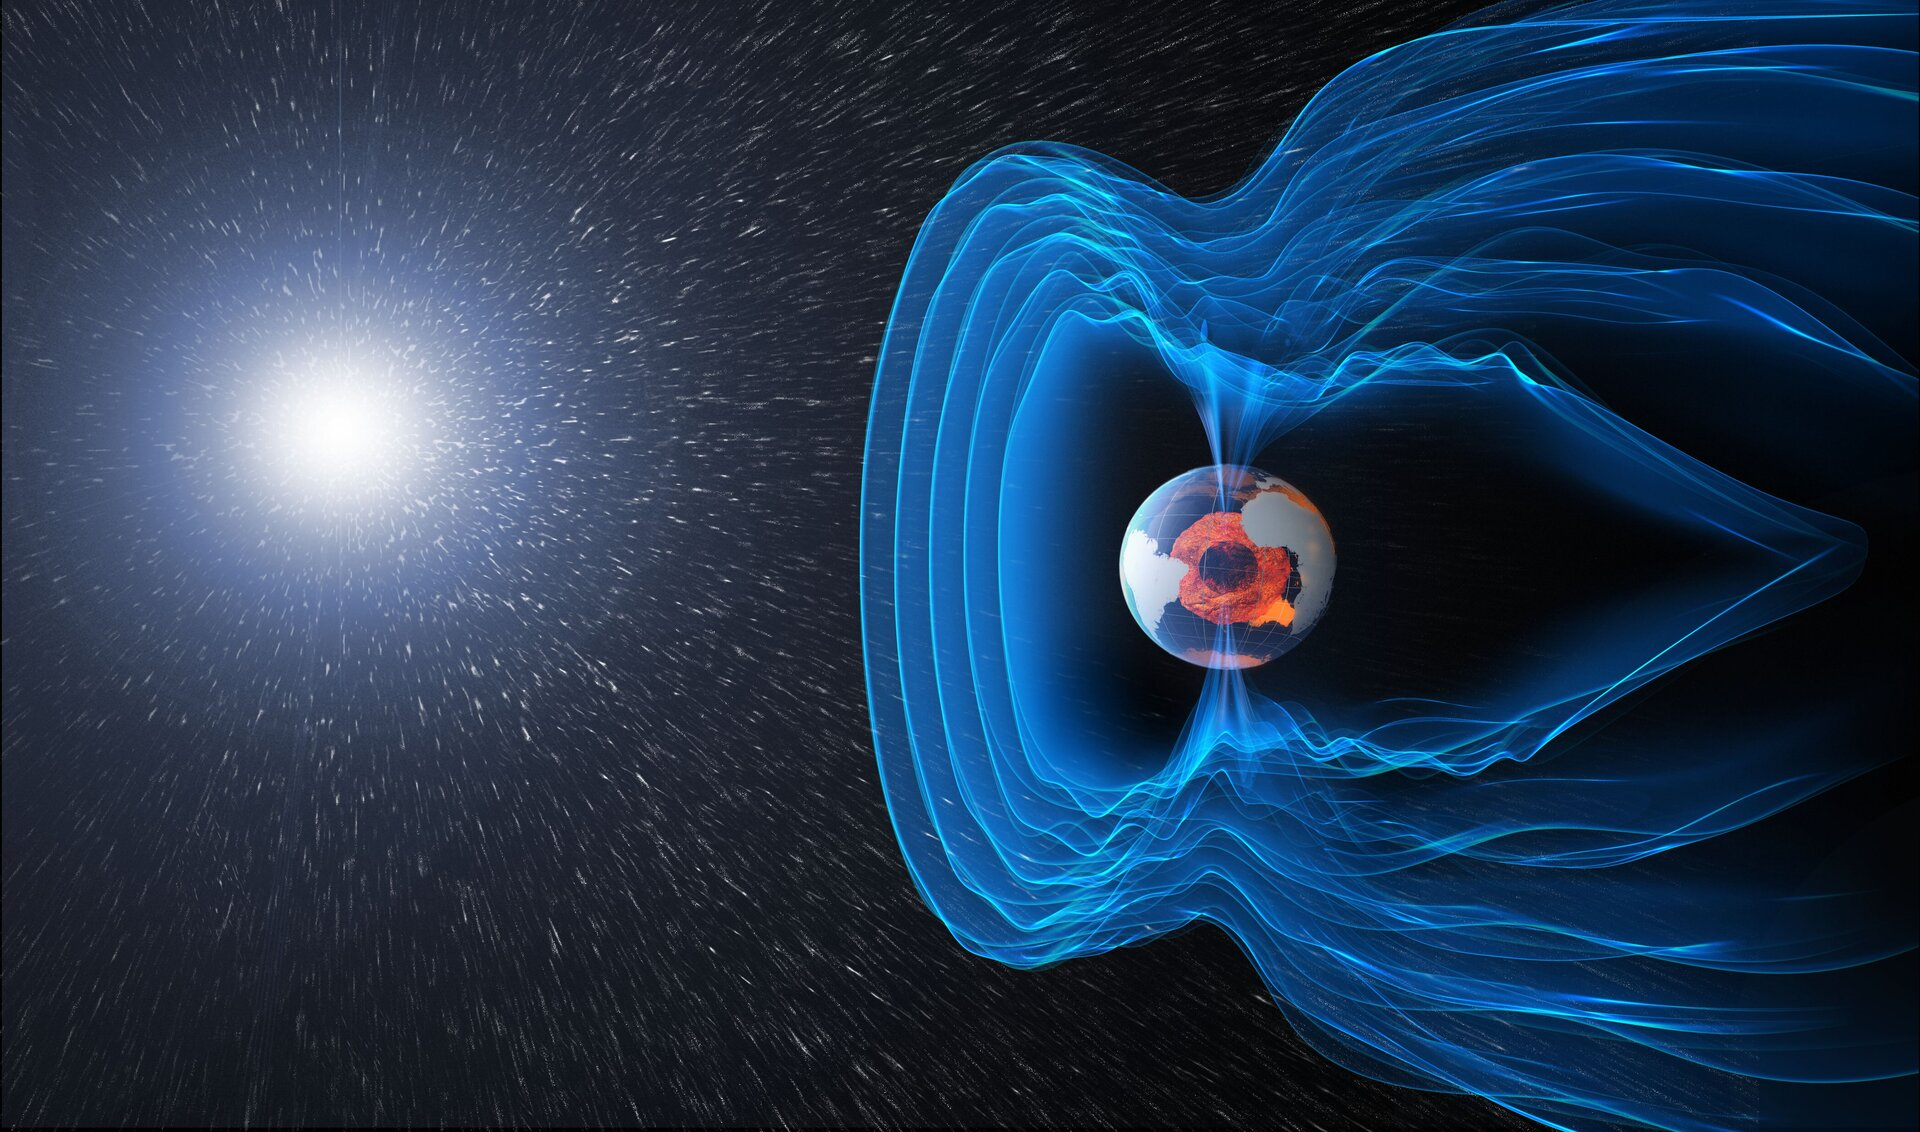
\includegraphics[width=1\textwidth]{images/cover1.jpg}
    \end{figure}

    % ---- Pousse le bloc suivant tout en bas de la page ----
    \vfill
    \noindent
    \begin{minipage}{0.48\textwidth}
        \raggedright
        Justine GARRAU \\         Pierre GUÉNO \\         Arthur LEBAS \\         Louann MONJARRET \\
        
    \end{minipage}
    \hfill
    \begin{minipage}{0.48\textwidth}
        \raggedleft
        Tuteurs : \\ Gautier NGUYEN \\ Antoine BRUNET \\ Guillerme BERNOUX
    \end{minipage}

\end{titlepage}